\documentclass[border=2mm]{standalone}
\usepackage{tikz}
\usepackage{pgfplots}
\pgfplotsset{compat=1.16, ticks=none}
\usepackage{amsmath}
\begin{document}
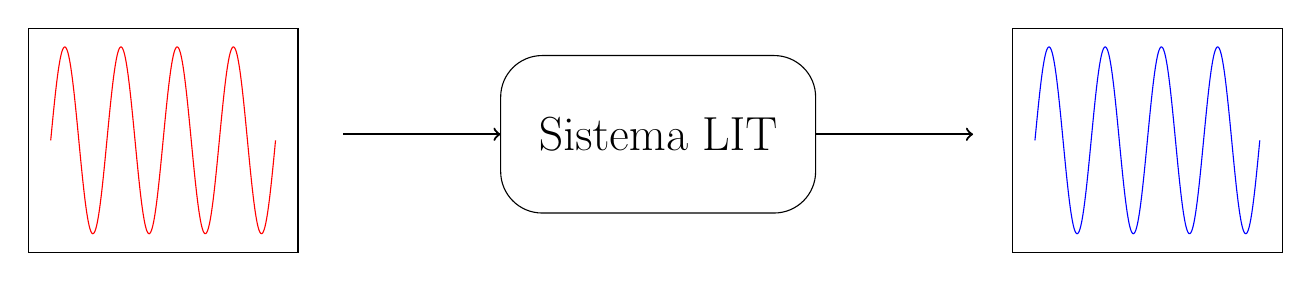
\begin{tikzpicture}[font=\LARGE]
    \draw [rounded corners=15pt] (0, 0) rectangle (4, 2) node [pos=0.5] {Sistema LIT};
    \draw [->, thick] (-2, 1) -- (0, 1);
    \draw [->, thick] (4, 1) -- (6, 1);
    \begin{axis}[
        xshift=-6cm, yshift=-0.5cm,
        scale=0.5,
        ]
        \addplot[domain=0:2*pi,samples=300,red]{sin(4*deg(x))};
    \end{axis}
    \begin{axis}[
        xshift=6.5cm, yshift=-0.5cm,
        scale=0.5,
        ]
        \addplot[domain=0:2*pi,samples=300,blue]{sin(4*deg(x))};
    \end{axis}
\end{tikzpicture}
\end{document}